\documentclass{book}

\usepackage{graphicx}
\usepackage[italian]{babel}
%\usepackage{listings}
%\usepackage[export]{adjustbox}
\usepackage{hyperref}
\usepackage{bohr}
\hypersetup{linktoc=all}

\begin{document}
    
\author{Giovanni Tosini}
\title{Fisica II}
\date{ }
\maketitle
\newpage
\tableofcontents
\newpage

\section{Introduzione}

Esistono due tipi di forze in assoluto:
\begin{itemize}
    \item forze attrattive
    \item forze repulsive
\end{itemize}
Queste forze si possono vedere anche nelle singole cariche elettriche, quelle con identica carica
si respingeranno, mentre quelle con carica opposta si attrarranno.

Esistono tre modalità per caricare un oggetto:
\begin{itemize}
    \item strofinio
    \item induzione
    \item contatto
\end{itemize}
Da notare che la carica non dipende dal meccanismo con cui viene creata, ma dai costituenti
della materia.
\begin{center}
    \bohr{10}{A}
    \setbohr{nucleus-radius=1.5em}    
\end{center}
Un atomo è composto da: protoni, neutroni ed elettroni. La differenza di dimensioni tra un protone
e un elettrono è di parecchi ordini di grandezza. La carica elettrica di un elettrone viene 
denominata "carica elementare", è tale perché si dice "quantizzata" essendo che si possono trovare solo
cariche multiple di essa. Inoltre il modulo della carica di un elettrone è equivalente alla carica di
 un protone, sebbene siano due particelle differenti.
 \begin{quote}
     \begin{math}
         |qe^-| = qe^+
     \end{math}
 \end{quote}
 La materia ordinaria è neutra, di conseguenza pure l'atomo è neutro, ovvero il centro di 
 simmetria del nucleo coincide con quello degli elettroni.

 Con lo strofinio vengono strappati gli elettroni meccanicamente, nel sistema isolato d'esempio
 (in un sistema isolato la carica totale Q si conserva) preso in questione. La carica dipenderà 
 dal potenziale di estrazione del materiale.

 Per induzione invece, un oggetto \begin{math}
     q^+
 \end{math} avvicinato a un oggetto neutro, porterà a una divisione di cariche nell'oggetto neutro 
 causato dall'induzione elettrostatica
 \begin{center}
     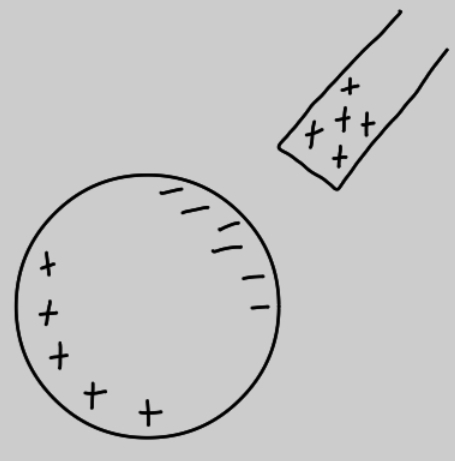
\includegraphics[width=0.5\textwidth]{induzione_elettrostatica.jpg}
 \end{center}

 \section{Elettrostatica nel vuoto (in assenza di materia dielettrica)}

Quando non c'è dipendenza dal tempo il campo elettrico e il campo magnetico sono separati.

\subsection{Interazione (forze) di Coulomb}

\begin{center}
    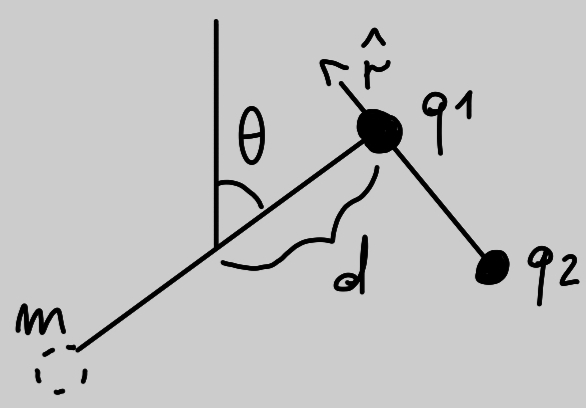
\includegraphics[width=0.5\textwidth]{coulomb.jpg}
\end{center}

\begin{itemize}
    \item m oggetto di massa m, trascurabile
    \item \begin{math}
        \theta
    \end{math} angolo
    \item $q_1$ e $q_2$ sono le cariche
    \item d la distanza
    \item r il versore
\end{itemize}

La forza esercitata lungo d sarà equivalente a:
\begin{quote}
    \begin{math}
        |\vec{F}|=k\frac{q_1q_2}{r^2}
    \end{math}
\end{quote}
Questo è un modello valido \textbf{esclusivamente} per cariche ferme nel vuoto. La costante k 
equivale a
\begin{quote}
    \begin{math}
        k=\frac{1}{4\pi\epsilon_0}
    \end{math}
\end{quote}
Di conseguenza la forza esercitata su $q_1$ sarà equivalente a
\begin{quote}
    \begin{math}
        \vec{F}=\frac{1}{4\pi\epsilon_0}\frac{q_1q_2}{r^{2}_{1,2}}
    \end{math}
\end{quote}

N.B.: \begin{itemize}
    \item l'unità di misura della carica equivale al Coulomb, q = [C].
    \item \begin{math}
        \epsilon_0
    \end{math} è la permeabilità sul vuoto (  costante dielettrica del vuoto)
    \item \begin{math}
        r_{1,2} = \vec{r}_{12} = \vec{r}_2 - \vec{r}_1
    \end{math}
    \item se \begin{math}
        q_1q_2
    \end{math} è positivo allora avremo a che fare con una forza repulsiva, se negativo attrattiva
\end{itemize}

\begin{center}
    \includegraphics*[width=0.5\textwidth]{coulomb_2.png}
\end{center}
\begin{center}
    \includegraphics*[width=0.5\textwidth]{coulomb_3.png}
\end{center}
Una carica $q_0$ in uno spazio vuoto, con attorno N cariche, sarà sotto l'effetto della somma della forza di tutte:
\begin{quote}
    \begin{math}
        \sum_{i = 1}^N \frac{q_iq_0}{4\pi\epsilon_0}\frac{\hat{r}_{i0}}{r_{{i0}^2}}
    \end{math}
\end{quote}
N.B.: \begin{itemize}
    \item l'unità di misura della forza è il Newton [N]
    \item \begin{math}
        \hat{r_{12}} = \hat{r_2 - r_1}
    \end{math}
\end{itemize}

\subsection{Campo elettrostatico}
\begin{quote}
    \begin{math}
        \vec{F_{q_0}} = q_0\vec{E}_i(\vec{r}_0)
    \end{math}
\end{quote}
dove
\begin{itemize}
    \item $\vec{E}$ è la sommatoria senza $q_0$
    \item $\vec{r}_0$ equivale a $\frac{1}{4\pi\epsilon_0}\frac{q_i}{r^2_{i0}}\hat{r}_i0$
    \item che a sua volta equivale a $\frac{\vec{F}_{q_iq_0}}{q_o}$
    \item $\vec{F}_{q_iq_0} = q_0\vec{E_i}$
    \item $\vec{F}_{tot} = q_0\sum \vec{E}_i$
\end{itemize}

Ogni carica genera un campo, ma un campo esiste anche in assenza di particelle
\begin{quote}
    \begin{math}
        \vec{E}(\vec{r}) = \frac{q}{4\pi\epsilon_0r^2}\hat{r}
        \newline\vec{E}_{tot}(r) = \sum\vec{E}_i = \sum \frac{q_i\hat{r}_{i0}}{4\pi\epsilon_0(r_i-r)^2}
        \newline\vec{F} = q\vec{E}
    \end{math}
\end{quote}
Definizione "operativa" di campo elettrico:
\begin{quote}
    \begin{math}
        \vec{E} = \frac{\vec{F}}{q} [\frac{N}{C}] = [\frac{V}{m}]
    \end{math}
\end{quote}

\subsection{Energia elettrostatica}

La forza elettrostatica è conservativa? Lo è se:
\begin{itemize}
    \item L non dipende dal percorso
    \item L in un percorso chiuso è nullo
    \item Esiste una funzione di energia potenziale U t.c. L da A->B è uguale a -$\Delta$U
\end{itemize}
\begin{center}
    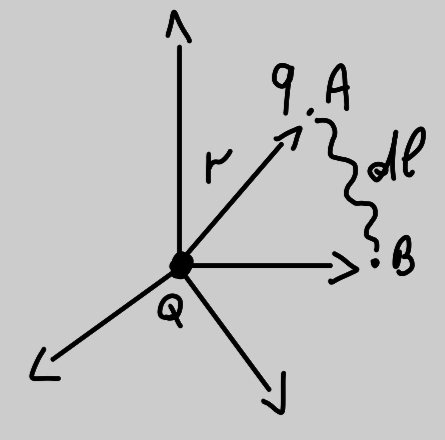
\includegraphics[width=0.5\textwidth]{energia_elettrostatica_1.jpg}
\end{center}
\begin{itemize}
    \item Q è la particella che genera il campo elettrico
    \item q invece è la particella che si sposta da A a B
    \item $dL = \vec{F}\vec{dl}$
    \item $dL = \frac{qQ}{4\pi\epsilon_0r^2}\hat{r}\vec{dl}$
\end{itemize}
$\hat{r}\vec{dl}$ non è nient'altro che la proiezione di $r$ su $dl$ ovvero $dr$
\newline Il lavoro da A a B invece equivale all'integrale
\begin{quote}
    \begin{math}
        L_{AB} = \int^B_A dL = \frac{qQ}{4\pi\epsilon_0} \int^B_A \frac{\hat{r}\vec{dl}}{r^2} = \int^{r_B}_{r_A} \frac{dr}{r^2} 4
        = -\frac{1}{r}|^{r_B}_{r_A}
    \end{math}
    che è uguale a 
    \begin{math}
        \frac{qQ}{4\pi\epsilon_0}(\frac{1}{r_A}-\frac{1}{r_B}) = -\Delta U\\
        \newline U_{carica q} = \frac{qQ}{4\pi\epsilon_0r}+c
    \end{math}
\end{quote}
L'unità di misura dell'energia potenziale è il Joule [J]
\newline $U_\infty = 0$ perché non ci sono cariche
\newline $U = \frac{qQ}{4\pi\epsilon_0r} = -(U_\infty-U_r) = -\Delta U$




\end{document}